\documentclass[a4paper]{scrartcl}
\usepackage[cm]{fullpage}
\usepackage{amsmath, amssymb, esint}
\usepackage{siunitx}
\usepackage[backend = biber, style = numeric-comp]{biblatex}

\usepackage{tikz, pgfplots}
\pgfplotsset{
    compat = 1.12,
    plot/.style = {
        axis lines = middle,
        clip = false
    },
    plot-scatter/.style = {
        only marks,
        error bars/.cd,
        x dir = both, y dir = both,
        x explicit, y explicit
    }
}

\begin{filecontents}{\jobname.bib}
@misc{FindDistributionParameters,
	url = {http://reference.wolfram.com/language/ref/FindDistributionParameters.html},
	year  = {2017},
	month = {mar},
	title = {FindDistributionParameters --- Wolfram Language Documentation}
}
@misc{bootstrap-analysis,
    url = {http://reference.wolfram.com/language/howto/PerformABootstrapAnalysis.html},
    year  = {2017},
    month = {mar},
    title = {Perform a Bootstrap Analysis --- Wolfram Language Documentation}
}
@article{Olive:2016xmw,
    author         = "Patrignani, C. and others",
    title          = "{Review of Particle Physics}",
    collaboration  = "Particle Data Group",
    journal        = "Chin. Phys.",
    volume         = "C40",
    year           = "2016",
    number         = "10",
    pages          = "100001",
    doi            = "10.1088/1674-1137/40/10/100001",
    SLACcitation   = "%%CITATION = CHPHD,C40,100001;%%"
}
\end{filecontents}
\addbibresource{\jobname.bib}

\begin{document}

\title{PHYS3112: Muon Lifetime}
\author{ \\ \\ }
\date{2017-03-27}
\maketitle

\section{Abstract}
By fitting a mixed distribution function to \(\Delta t\)s between scintillator detections of atmospheric muons, we obtain a muon lifetime of \(\tau = \SI{2.06 \pm 0.19}{\micro\second}\). This is in agreement with the \SI{2.197}{\micro\second} value in the literature\cite{Olive:2016xmw}.

\section{Materials and Methods}
Please refer to the operating instructions of the experiment and the prework.

The photomultiplier tube (PMT) produced ringing (damped oscillations) for every muon detection that lasted about \SI{200}{\nano\second}. This could potentially produce spurious detections or inaccurate timings during the ringing, so any timings less than \SI{200}{\nano\second} was ignored from the analysis. The discriminator's threshold voltage was set such that all but the largest of ringings produced a double detection, however.

From our prework, we expect the timings to follow an exponential distribution with lifetime \(\tau\) representing the decays, mixed (CDFs added together) with an approximately uniform distribution representing multiple muons travelling through the scintillator (``through-going''). Since we are only considering timings between \SI{200}{\nano\second} and \SI{20000}{\nano\second}, the distribution is appropriately truncated. \(r\) is the rate through-going muons are detected per decay event. Its PDF is:
\[\frac{r}{(\SI{19800}{\nano\second}) (r + 1)} + \frac{e^{-\frac{\Delta t}{\tau}}}{(r + 1) \left(e^{-\frac{\SI{200}{\nano\second}}{\tau}} - e^{-\frac{\SI{20000}{\nano\second}}{\tau}}\right) \tau}\]

Our timings were then fitted to this distribution by maximising the log likelihood\cite{FindDistributionParameters}. Standard errors were produced by performing a bootstrap analysis\cite{bootstrap-analysis}.

\section{Results}
\begin{figure}
    \centering
    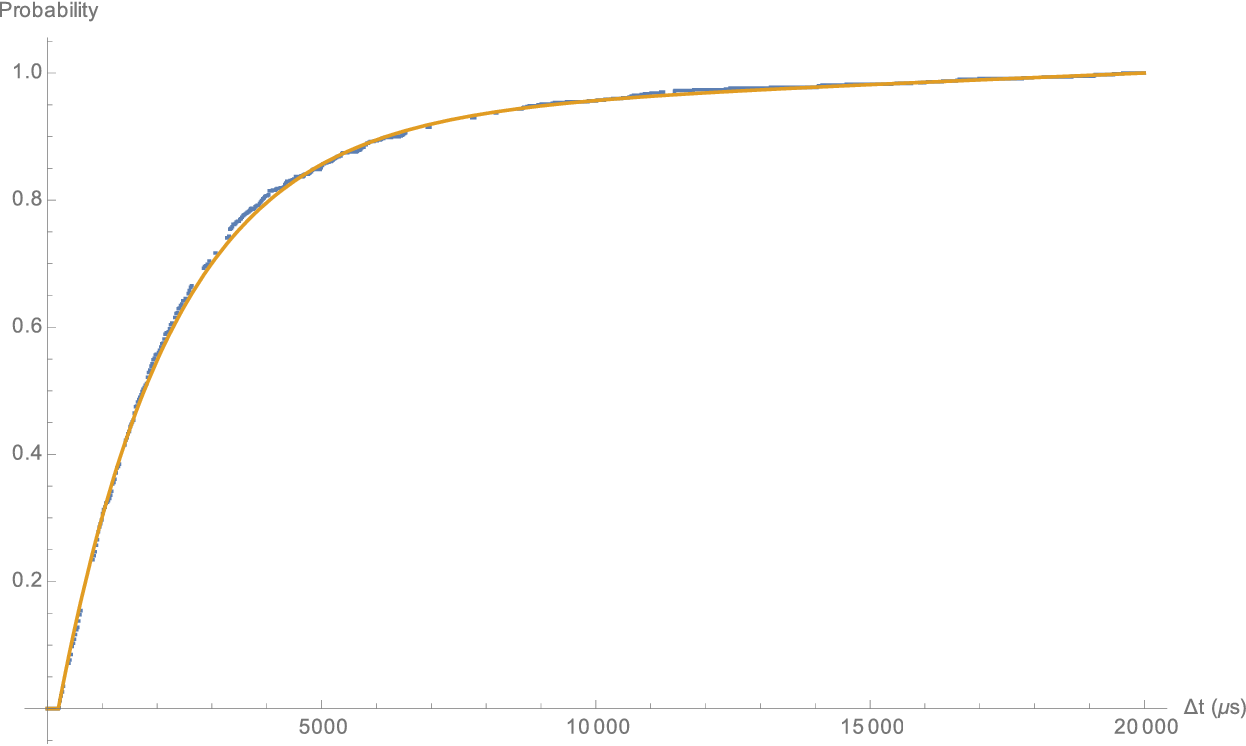
\includegraphics[height = 10cm]{cdf.png}
    \caption{ \(\Delta t\) CDF of double detections (Blue: Samples; Red: Filtered curve)}
    \label{fig:cdf}
\end{figure}

\SI{168183}{} detections events were recorded over \SI{11425}{\second}, which is an average rate of \SI{14.721}{\per\second}. Of these detections, 962 were double detections, of which 798 of them had delays of not less than \SI{200}{\nano\second}. This resulted in a fitted distribution with parameters \(r = \SI{0.075 \pm 0.034}{}\) and \(\tau = \SI{2.06 \pm 0.19}{\micro\second}\).

The CDFs of the data and the fitted distribution are shown in Figure \ref{fig:cdf}. A Pearson \(\chi^2\) test resulted in a p-value of 0.44 for rejecting the null hypothesis (that the data does not fit the distribution).

\section{Discussion}
Our detection rate of \SI{14.721}{\per\second} matches the \SI{15}{\per\second} rate mentioned in the student notes, which means that the detections are reasonably likely to be muons. Our decay lifetime of \SI{2.06 \pm 0.19}{\micro\second} also matches the \SI{2.197}{\micro\second} value in the literature\cite{Olive:2016xmw}.

Both visual examination of the fitted CDF and the Pearson \(\chi^2\) test suggest the distribution matches the data.

While this is a good result, the precision of our value of \(\tau\) leaves much to be desired. The experiment would have benefited from a much longer measurement duration (our's was only a tad over 3 hours), as well as a larger detection volume, so we could have more data points to work with and improve precision.

\section{Conclusion}
\emph{(From abstract)} By fitting a mixed distribution function to \(\Delta t\)s between scintillator detections of atmospheric muons, we obtain a muon lifetime of \(\tau = \SI{2.06 \pm 0.19}{\micro\second}\). This is in agreement with the \SI{2.197}{\micro\second} value in the literature\cite{Olive:2016xmw}.

This shows that our results and experimental setup were reasonable, though our low precision on the lifetime suggests things can be improved.

\printbibliography

\end{document}